\colorlet{species background color}{black!15}
\tikzset{
    x={1pt},
    y={-1pt},
    species border/.style={
        line width={1pt},
        shorten <={-1pt / 2 + 0.05pt},
        shorten >={-1pt / 2 + 0.05pt},
    },
    species background/.style={
        fill=species background color,
        draw=species background color,
        line width={1pt},
        rounded corners,
    },
    species label/.style={
        font=\bfseries,
        midway,
        anchor=north,
        align=center,
        yshift=-10,
    },
    branch/.style={
        draw={#1},
        line width={0.5pt},
    },
    transfer branch/.style={
        branch={#1},
        -Stealth,
    },
    loss/.style={
        draw={#1}, cross out, thick,
        line width={0.5pt},
        inner sep=0pt,
        outer sep=0pt,
        minimum width={3},
        minimum height={3},
    },
    extant gene/.style 2 args={
        circle, fill={#1},
        outer sep=0pt, inner sep=0pt,
        minimum size={3},
        label={
            [font={\strut\color{#1}},
                align=center,
                inner xsep=0pt, inner ysep=2pt,
                outer xsep=0pt, outer ysep=0pt]
            below:#2
        },
    },
    extant gene/.default={black}{},
    branch node/.style={
        draw={#1}, fill={species background color!50!white},
        align=center,
        font={\color{#1}},
        outer sep=0pt, inner xsep=0pt, inner ysep=2pt,
        line width={0.5pt},
    },
    branch node/.default={black},
    speciation/.style={
        branch node={#1}, rectangle, rounded corners,
        inner xsep=4pt,
        minimum width={8},
        minimum height={8},
    },
    duplication/.style={
        branch node={#1}, rectangle,
        inner xsep=4pt,
        minimum width={8},
        minimum height={8},
    },
    horizontal gene transfer/.style={
        branch node={#1}, chamfered rectangle,
        chamfered rectangle sep={8 / 2.4},
        inner xsep=2pt,
        inner ysep=-1pt,
        minimum width={8},
        minimum height={8},
    },
}
\definecolor{reccolor0}{HTML}{000000}
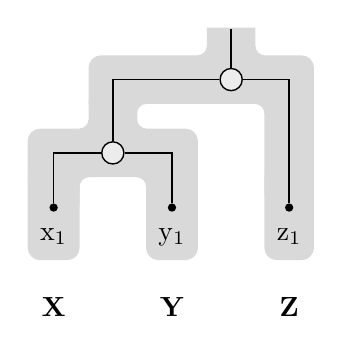
\begin{tikzpicture}
% background
\path[species background] (22.012999999999998,26.5) -- (22.012999999999998,10) -- (64.776,10) [sharp corners] -- (64.776,0) -- (81.276,0) [rounded corners] -- (81.276,10) -- (102.449,10) [sharp corners] -- (102.449,53.0) [rounded corners] -- (85.526,63.0) -- (85.526,26.5) -- (38.513,26.5) [sharp corners] -- (38.513,36.5) -- cycle;
\path[species background] (0,53.0) -- (0,36.5) -- (22.012999999999998,36.5) [sharp corners] -- (22.012999999999998,26.5) -- (38.513,26.5) [rounded corners] -- (38.513,36.5) -- (60.525999999999996,36.5) [sharp corners] -- (60.525999999999996,53.0) [rounded corners] -- (42.763,63.0) -- (42.763,53.0) -- (17.762999999999998,53.0) [sharp corners] -- (17.762999999999998,63.0) -- cycle;
\path[species background] (0,53.0) -- (0,83.0) -- (17.762999999999998,83.0) -- (17.762999999999998,53.0);
\path[species background] (42.763,53.0) -- (42.763,83.0) -- (60.525999999999996,83.0) -- (60.525999999999996,53.0);
\path[species background] (85.526,53.0) -- (85.526,83.0) -- (102.449,83.0) -- (102.449,53.0);
% species
\path[species border] (22.012999999999998,26.5) -- (22.012999999999998,10) -- (64.776,10) -- (64.776,0);
\path[species border] (102.449,53.0) -- (102.449,10) -- (81.276,10) -- (81.276,0);
\path[species border] (38.513,26.5) -- (38.513,26.5) -- (85.526,26.5) -- (85.526,53.0);
\path[species border] (0,53.0) -- (0,36.5) -- (22.012999999999998,36.5) -- (22.012999999999998,26.5);
\path[species border] (60.525999999999996,53.0) -- (60.525999999999996,36.5) -- (38.513,36.5) -- (38.513,26.5);
\path[species border] (17.762999999999998,53.0) -- (17.762999999999998,53.0) -- (42.763,53.0) -- (42.763,53.0);
\path[species border] (0,53.0) -- (0,83.0) -- node[species label] {X} (17.762999999999998,83.0) -- (17.762999999999998,53.0);
\path[species border] (42.763,53.0) -- (42.763,83.0) -- node[species label] {Y} (60.525999999999996,83.0) -- (60.525999999999996,53.0);
\path[species border] (85.526,53.0) -- (85.526,83.0) -- node[species label] {Z} (102.449,83.0) -- (102.449,53.0);
% gene branches
\path[branch={reccolor0}] (73.026,14) -- (73.026,0);
\draw[branch={reccolor0}] (30.262999999999998,26.5) |- (68.776,18.25) (77.276,18.25) -| (93.9875,53.0);
\path[branch={reccolor0}] (30.262999999999998,40.5) -- (30.262999999999998,26.5);
\draw[branch={reccolor0}] (8.881499999999999,53.0) |- (26.012999999999998,44.75) (34.513,44.75) -| (51.644499999999994,53.0);
\path[branch={reccolor0}] (8.881499999999999,63.0) -- (8.881499999999999,53.0);
\path[branch={reccolor0}] (51.6445,63.0) -- (51.644499999999994,53.0);
\path[branch={reccolor0}] (93.9875,63.0) -- (93.9875,53.0);
% gene transfers
% events
\node[speciation={reccolor0}] at (73.026,18.25) {};
\node[speciation={reccolor0}] at (30.262999999999998,44.75) {};
\node[extant gene={reccolor0}{x\textsubscript{1}}] at (8.881499999999999,64.5) {};
\node[extant gene={reccolor0}{y\textsubscript{1}}] at (51.6445,64.5) {};
\node[extant gene={reccolor0}{z\textsubscript{1}}] at (93.9875,64.5) {};
\end{tikzpicture}
